An active front-end (AFE) converter, is a grid interface converter that
transfers power between an energy source and the utility grid, and between the
utility grid and a load. It's a controllable rectifier that can exchange power
between AC and DC power in both directions, and can regenerate power to the
mains to reduce power costs.
\section{Problem Statement}
My team at Statcon Electronics India Ltd has been focusing on on enhancing the
efficiency and performance of front-end converters. Presently, most active
front-end converters utilize Silicon Controlled Rectifiers (SCRs) for
rectification, employing a conventional 6-pulse converter configuration. My
task was to explore and design a active front-end using Insulated Gate Bipolar
Transistors (IGBTs) as alternatives to SCRs in the rectification process.

The primary objective of this project is to investigate the feasibility and
advantages of using IGBTs instead of SCRs for rectification in active front-end
converters. Specifically, we aim to implement a Space Vector Pulse Width
Modulation (SVPWM) technique to control the IGBTs effectively. This technique
offers precise control over the switching patterns of the IGBTs, allowing for
optimized power conversion and reduced harmonic distortion.

Furthermore, the project involves the development of a sophisticated control
algorithm to manage the operation of the IGBTs. This algorithm must facilitate
seamless transition between pulling current from the grid (rectification mode)
and supplying current to the grid (regeneration mode). The control system
should ensure stable and efficient operation under varying load conditions
while maintaining compliance with grid standards and regulations.

\section{Overview}
A three-phase AC to DC converter is essential for many power electronics system
such as Variable frequency drive (VFD), battery charger, uninterruptible power
supplies (UPS).

Traditionally diode rectifiers or thyristor rectifier are used for AC to DC
conversion, both these rectifiers behave as non- linear loads. The currents
drawn by the rectifiers include a fundamental component and harmonic
components. The voltage drop across the line inductance due to the harmonic
currents distorts the mains voltage. Consequently, the other loads connected to
the mains are also fed with a distorted voltage.

\subsection{Traditional Rectifier}
Diode rectifier, depicted in Figure~\ref{fig:diode_rectifier}, produces a
constant DC voltage, which is a function of the system voltage. A thyristor
based rectifier can produce a variable DC voltage. But, both these topology
behave as non-linear loads.

\begin{figure}[h]
    \centering
    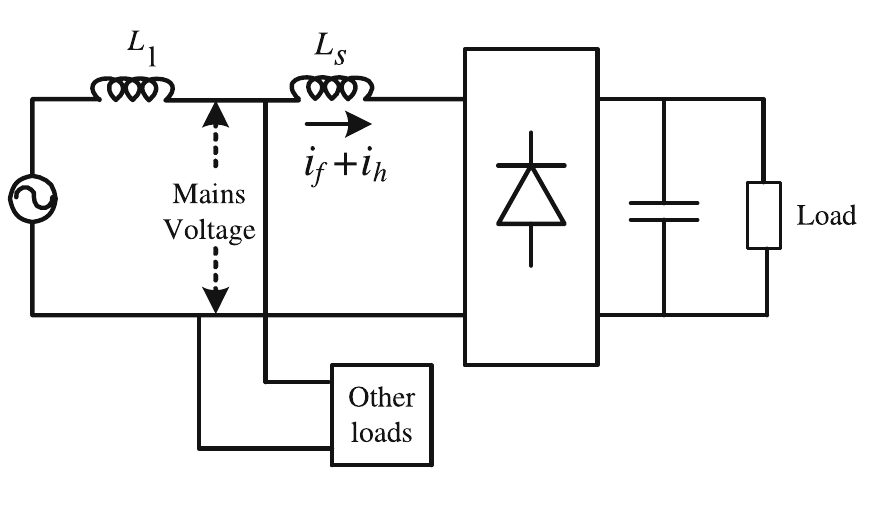
\includegraphics[width=\textwidth]{Diode Rectifier.png}
    \caption{AC to DC Conversion using Diode Rectifier.}
    \label{fig:diode_rectifier}
\end{figure}

\subsection{IGBT Rectifier}
\begin{figure}[h]
    \centering
    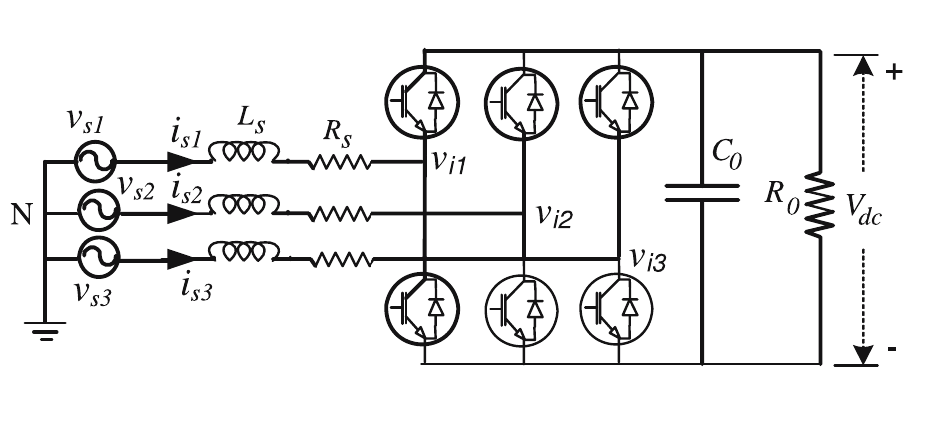
\includegraphics[width=\textwidth]{IGBT Rectifer.png}
    \caption{Schematic diagram of
        a front-end converter (FEC)}
    \label{fig:igbt_rectifier}
\end{figure}
\noindent
IGBT Rectifer, depicted in Figure~\ref{fig:igbt_rectifier}, draws near
sinusoidal current from grid. The power factor as well as DC Voltage can be
adjusted. Since it is connected to line side it is called line side or front
end converter.

The converter consists of a three-phase bridge, a high capacitance on the dc
side and a three-phase inductor in the line-side. The voltage at the mid point,
$V_i$ is pulse width modulated (PWM) in nature. The voltage consists of a
fundamental component (at line frequency) besides harmonic components around
the switching frequency of the converter. Being at high frequencies, these
harmonic components are well filtered by the line inductor. Hence the current
is near sinusoidal. The fundamental component of $V_i$ controls the flow of
real and reactive power.

\subsection{Vector Control}
Vector control is a popular method for control of three-phase induction motors.
The basic idea of this scheme is to control the flux producing and the
torque-producing components of motor current. The outer control loop controls
the speed of the motor, while the inner loop controls the components of current
vector, which correspond to torque and flux. Similar control approach can be
used for FEC also. Here, the three-phase grid voltages and line currents are
converted into an equivalent two-phase system, called stationary reference
frame . These quantities are further transformed into
a reference frame called synchronous reference frame, which revolves at the
grid frequency .

\subsection{Space Vector Modulation}
This technique, also known as Space Vector Pulse Width Modulation (SVPWM), is a
method used to generate the switching signals for the IGBTs in the AFE
converter. It offers precise control over the IGBT switching patterns by
synthesizing the desired output voltage as a combination of multiple voltage
vectors. SVM has eight space vectors, other space vectors are synthesized by
alternating active and zero vectors over a switching period.

\section{Challenges}
I faced many challenges in developing a Active front-end converter. Firstly,
distinguishing between Sinusoidal Pulse Width Modulation (SPWM) and Space
Vector Pulse Width Modulation (SVPWM) posed confusion due to their perceived
similarity in operational principles. Secondly, reconciling the non-zero
resultant vector in SVPWM with the traditional understanding of three-phase
systems, where the vector sum equals zero, required conceptual clarification to
ensure accurate system design and analysis. Another challenge was comprehending
how rectification and regeneration can occur through the same IGBT bridge, as
it involved bidirectional power flow management. Additionally, not knowing how
to write code in MATLAB was another challenge, but learning it opened up new
possibilities for simulating and analyzing our AFE converter designs.